% Curvature from gluing flat equilateral triangles around a single vertex.
% Five triangles leave a gap and the surface cones up, six lie flat,
% seven have no room in the plane and the surface buckles.
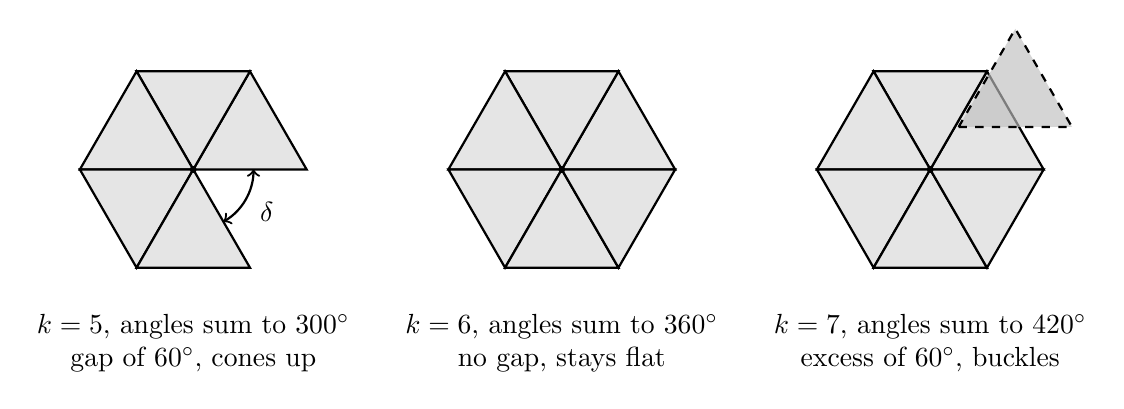
\begin{tikzpicture}[thick, scale=0.9]
  \def\R{1.6}

  % k = 5, positive deficit
  \begin{scope}
    \foreach \i in {0,...,4} {
      \fill[gray!20] (0,0) -- ({\i*60}:\R) -- ({(\i+1)*60}:\R) -- cycle;
      \draw          (0,0) -- ({\i*60}:\R) -- ({(\i+1)*60}:\R) -- cycle;
    }
    \draw[<->] (300:0.85) arc (300:360:0.85);
    \node at (330:1.2) {$\delta$};
    \fill (0,0) circle (1.4pt);
    \node[align=center] at (0,-2.45)
      {$k=5$, angles sum to $300^\circ$\\ gap of $60^\circ$, cones up};
  \end{scope}

  % k = 6, zero deficit
  \begin{scope}[xshift=5.2cm]
    \foreach \i in {0,...,5} {
      \fill[gray!20] (0,0) -- ({\i*60}:\R) -- ({(\i+1)*60}:\R) -- cycle;
      \draw          (0,0) -- ({\i*60}:\R) -- ({(\i+1)*60}:\R) -- cycle;
    }
    \fill (0,0) circle (1.4pt);
    \node[align=center] at (0,-2.45)
      {$k=6$, angles sum to $360^\circ$\\ no gap, stays flat};
  \end{scope}

  % k = 7, negative deficit
  \begin{scope}[xshift=10.4cm]
    \foreach \i in {0,...,5} {
      \fill[gray!20] (0,0) -- ({\i*60}:\R) -- ({(\i+1)*60}:\R) -- cycle;
      \draw          (0,0) -- ({\i*60}:\R) -- ({(\i+1)*60}:\R) -- cycle;
    }
    \draw[dashed, fill=gray!50, fill opacity=0.65]
      (0.4,0.6) -- ++(0:\R) -- ++(120:\R) -- cycle;
    \fill (0,0) circle (1.4pt);
    \node[align=center] at (0,-2.45)
      {$k=7$, angles sum to $420^\circ$\\ excess of $60^\circ$, buckles};
  \end{scope}
\end{tikzpicture}
